%%%%%%%%%%%%%%%%%%%%%%%%%%%%%%%%%%%%%%%%%%%%%%%%%%%%%%%%%%%%%%%%%%%%%%%%%%%%%%%%
% Template for ASPLOS papers.
%
% History:
% 
% ASPLOS originally used jpaper.cls for submission but required acmart.cls for the
% final camera-ready version. To avoid a change in format, starting ASPLOS 2024 Fall 
% cycle, both the submission and the camera-ready versions started using acmart.cls.
%
%%%%%%%%%%%%%%%%%%%%%%%%%%%%%%%%%%%%%%%%%%%%%%%%%%%%%%%%%%%%%%%%%%%%%%%%%%%%%%%%%%

% use the base acmart.cls version 1.92
% use the sigplan proceeding template with the default 10 pt fonts
% nonacm option removes ACM related text in the submission. 
\documentclass[nonacm,sigplan]{acmart}

% enable page numbers
\settopmatter{printfolios=true}

% make references clickable 
\usepackage[]{hyperref}

\begin{document}

\title{CacheInf: Collaborative Edge-Cloud Cache System for Efficient Robotic Visual Model Inference}

%\author{...} % removed for anonymity

\begin{abstract}
  Placeholder
  Placeholder
  Placeholder
  Placeholder
\end{abstract}

\maketitle % should come after the abstract
\pagestyle{plain} % should come right after \maketitle


\section{Introduction}
Visual information is vital for various robotic tasks deployed on real-world edge devices (typically mobile robots), such as TODO. 
And as a major visual information processing method, fast visual model inference is important for the real-world robotic tasks to timely respond to environment changes. 
Unfortunately, the mobile robots often suffer slow visual model inference, because they are typically limited in computation power and suffer from limited and unstable wireless network bandwidth, making both local computation slow and naively offloading the computation to GPU servers slow.


To tackle this problem, we have the following two observations:
1. the robotic visual model mostly leverages local operators (i.e., computation results relies on local geometries); 
2. the images for robotic visual model inference are typically continual.
These imply that between visual model inference on consecutive images in visual robotic tasks, part of the previous computed results of local operators can be cached and reused, providing opportunity to both reduce local computation time and reduce transmission data volume, accelerating the overall visual model inference.

% The cached previous computed results, 
% Once reusable cache is identified, we can not only reuse the local cache to reduce local computation time, but also reuse the remote cache (e.g., the server side from the robot's perspective) to reduce transmission data volume, accelerating the overall visual model inference.

Based on these observations, we propose CacheInf, a collaborative edge-cloud cache system for efficient robotic visual model inference.
Given a continuous stream of visual input in a robotic visual task, CacheInf analyses the overlapping area between consecutive inputs;
based on the portion of overlapping area (reusable cache) and the current estimated wireless network bandwidth, CacheInf schedules on the action between reusing local cache to reduce local computation time and reusing the remote cache (e.g., the cache at the GPU server side from the robot's perspective) to reduce transmission time, to ultimately reduce the overall visual model inference time.
% Schedule cache and offloading...
% Reduce data volume transmission in offloading at higher bandwidth...
% At low bandwidth where offloading is not feasible, reduce local computation time...

The design of CacheInf is non-trivial.
The first challenge is to transform cached results to local computation acceleration.
While the cached result of overlapping areas can be reused and the corresponding computation can be skipped, the sparse and fragmented remaining area can not be computed on local operators which are typically highly optimized for dense local geometries and outperform their counterparts for sparse local geometries (e.g., TODO).
To make use of these highly optimized local operators, in CacheInf we search for a minimal set of rectangles that covers the uncached areas, split and combine them to a new rectangle while preserving local geometries and use it as a temporary input for the local operators whose computed result can be broken up and combined with the cache to form the correct result.
We also profile the cost of this process and would choose to ignore cache when the cached portion is too small to bring acceleration.

The second challenge is how to reduce the cache memory consumption, especially at the robot side which typically has a tight GPU memory budget.
In visual models, the computation results of local operators typically consumes significantly more memory that the parameters of local operators and naively caching all the computation result can lead to XX times memory consumption in our evaluation.

We observe that in visual models, the computation result of a local operator often serves as the input of another local operator where local geometries are kept. 
Thus in the cached scenario, the computation result of the combined rectangle of uncached areas can be directly passed to the following local operators without loss of information, and cache of the previous computation result between the two operators can be abandoned to reduce memory consumption.
We greedily search for a set of continual local operators whose starting and ending operators incur the least memory consumption when caching their computation results, so as to minimize cache memory consumption.

The third challenge is under various distribution scenarios of cache (e.g., all cache is located at local or the remote GPU server), how to fully utilize the cache for acceleration.
For example, when all cache is located at local due to previous limited wireless network bandwidth and we currently have a suitable wireless network bandwidth to offload computation to the remote GPU server, directly offloading all of the input means abandoning all local cache, damaging the potential gain of cache.

To tackle this problem, we integrate a recent offloading paradigm named Intra-DP (TODO: cite arxiv name): during visual model inference on an image, Intra-DP enables splitting of the input of local operators at the dimension of columns and assign different splits to the local robot and the remote GPU server for computation, so that local computation and data transmission of one image can be parallelized.
Under this paradigm, we can partially leverage the local cache to compute on a split of the input which leads to faster local computation and also reduced transmission data volume, to better utilize the existing cache. 
We extend the scheduler of Intra-DP to further consider the potential acceleration with cache and combine the heuristics about the previous two challenges into a new scheduling algorithm named XXX.

We implemented CacheInf using python and pytorch on Ubuntu20.04. 
To efficiently combine uncached areas into a new rectangle and recover this rectangle to correct result, we implemented these two operations as cuda kernel using taichi for faster parallel computation on GPU.
Our baselines include plain local computation, a state-of-the-art computation offloading system named TODO and our self-modified counterpart with cache enabled and Intra-DP.
Our datasets include the standard video datasets of TODO from torchvision.
We evaluated CacheInf on a four-wheel robot equipped with a Jetson NX Xavier that is capable of computing locally with the low power consumption GPU and a PC equipped with an Nvidia 2080ti GPU as the remote GPU server.
Extensive evaluation on various visual models and wireless network bandwidth circumstances shows that:
\begin{itemize}
    \item CacheInf is fast. Among the baselines, CacheInf reduced the end-to-end inference time by XX\% to XX\%.
    \item CacheInf saves energy. Among the baselines, CacheInf reduced the average energy consumed to complete inference on one image by XX\% to XX\%.
    \item CacheInf is also memory-efficient. The above advantages were obtained by only incurring XX\% to XX\% increase in memory consumption for CacheInf.
\end{itemize}

The major contribution of this paper is our new paradigm of using cached computation results to accelerate visual modified inference on a continuous stream of input images on robots and the corresponding scheduling algorithm TODO.
The resulting system, CacheInf, accelerates both local computation on the robot and the data transmission while offloading the computation to the remote GPU server by collaboratively considering and reusing cached computation results on both the robot and the server.
The accelerated visual model inference and the reduced power consumption will make real-world robots more performant on various robotic tasks and nurture more visual models to be deployed in real-world robots.
The source code and evaluation logs of CacheInf is available at TODO.

The rest of the paper is organized as follows TODO.



\section{Background}
\subsection{Robotic Tasks and Visual Models}

vision information and fast visual model inference are important for the robotic tasks

Visual models often use local operators; introduce local operators and non-local operators.

\subsection{Resource Limitations of Robots}
Computation power; wireless network

\subsection{Related Work}
offloading methods; intra-DP

Cache related (Guan will take it)

\section{System Overview}
The chapter presents an overview of the design of CacheInf.

\subsection{Working Environment and Metrics}
We assume that the working scenario of CacheInf is a mobile robot performing robotic tasks in a real-world field which requires real-time visual model inference on the continuous image stream captured from the on-board camera, to achieve real-time response to various environment changes.
The robot itself is equipped with low-power-consumption gpu to perform visual model inference which is slow and consumes too much power; it has wireless network access to a remote powerful GPU server that provides opportunity of acceleration, but the connection suffers from limited and unstable wireless network bandwidth.

While the requirements of real-time inference does not necessarily imply the requirement of high inference frequency, we measure the real-time metric by the average end-to-end inference latency when the robot is seamlessly performing inference, which leads to high inference frequency; the power consumption is also measured by average power consumption to finish inference on each image in the same scenario.

\subsection{Architecture of CacheInf}
To reduce inference latency by reusing cached previous computation results to both reduce local computation time and transmission time of offloading, CacheInf basically consists of three blocks: a scheduler, a cache tracker and an executor (TODO fix the names).

\begin{figure*}[!htb]
    \centering
    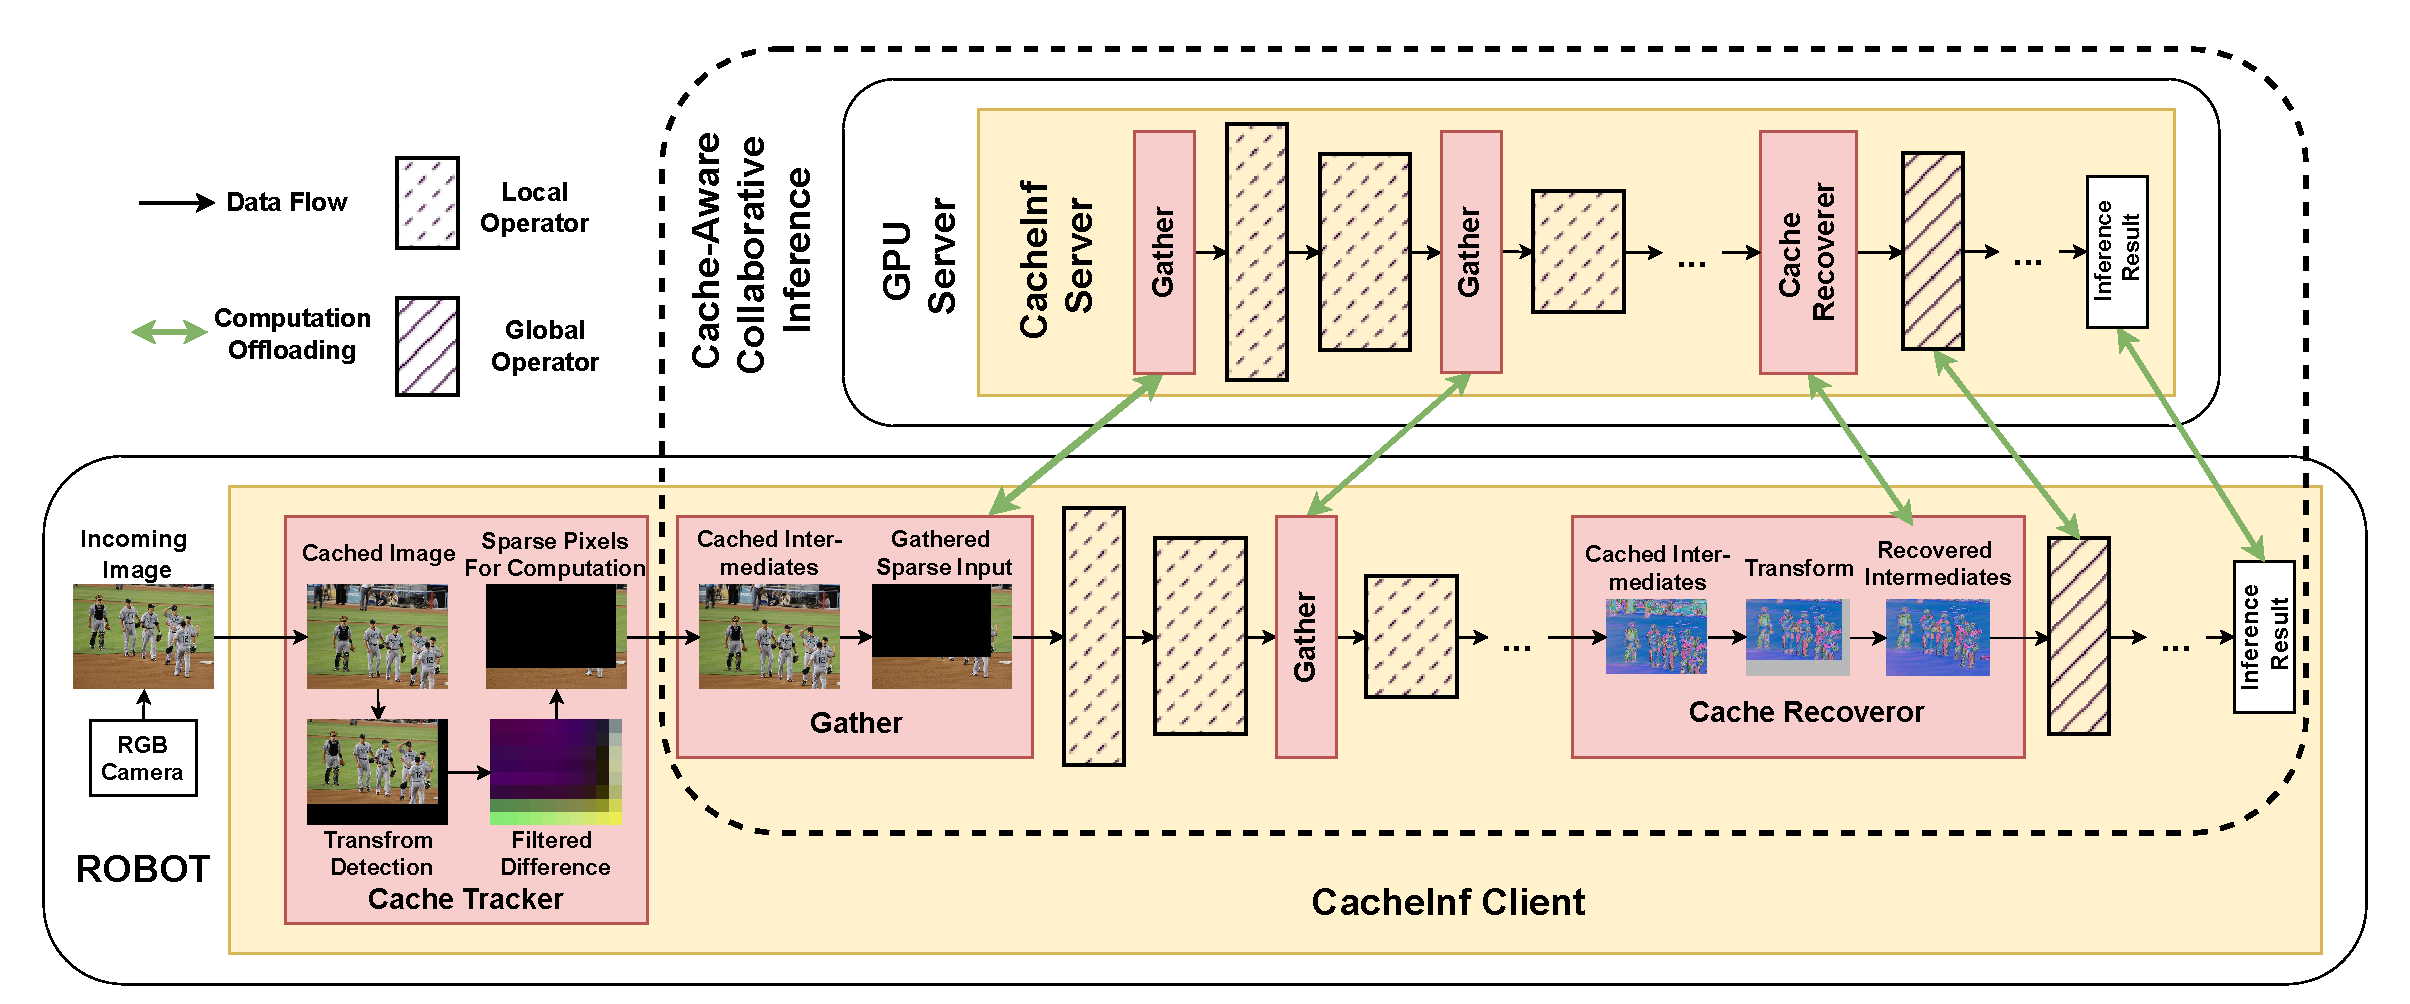
\includegraphics[width=\linewidth]{fig/overview.pdf}
    \caption[track]{Architecture and working process of CacheInf. TODO...}
    \label{fig:overview}
\end{figure*}

\subsubsection{Scheduler (TODO fix the names)}
During the initialization stage of the robotic task and CacheInf, CacheInf is granted access to the visual model and an initial input image and we mainly greedily pre-compute a schedule of various situations at this stage, since scheduling at runtime affects the real-time performance of the robotic task.
We first profile the model at both the robot and the remote GPU server to gather information  including shapes of the computation intermediates, the execution time of each operator (e.g., convolution, linear, etc.) on various scale of the input (e.g., from one tenth of the image to full scale of the image), the local property of each operator (i.e., whether the operator performs local computation) and so on.

Based on the above information, CacheInf finds sets of continuous local operators and assign the operators with smallest output sizes to be the operators to cache their computation results to reduce memory consumption of cache.
Then we coarsely iterate through the possible wireless network bandwidth, distribution of cache between the robot and the server and the portion of reusable cache and greedily compute a plan of whether to compute on cache and the portion of local computation and offloaded computation at the server at the reduced transmission data volume reusing cache.
We use the greedy strategy because we assume that both the wireless network bandwidth and the portion of reusable cache is unpredictable in the real-world scenario.
Note that the precomputed schedule can be reused for a same visual model with the same settings. 

\subsubsection{Cache Tracker}
At runtime, the selected operators at the previous stage will cache their computation results and the cache tracker identifies the reusable portion of such cached computation results.
Given an input image, we extract and store its features using classic computation vision methods (we choose Flann algorithm in our implementation, which is state-of-the-art).
For a current next image, we also extract and store its features and match them with the previous features (e.g., using KNN algorithm) and compute a perspective transform between the two images, which transforms the previous image such that the transformed previous image partially overlaps the current image and the non-overlapping areas are also marked.
The features of the previous images is then discarded.
The same transform can also be applied to the cached computation results since they are computed by local operators that keep the local geometries of the input image, and thus the reusable cached computation results are identified.
Note that the computation involved in this process is light-weight compared with the visual model inference that typically involves hundreds of operators.

\subsubsection{Executor (TODO fix the names)}
The executor is responsible to actually select and execute an plan based on results of the above two processes at runtime.
First, we further estimate the actual possible speedup by reusing cache, because the areas without cache needed for computation are often sparse and fragmented.
We cluster the areas without cache into different nearest clusters and compute minimum bounding boxes for each of the clusters;
then we greedily break up and recombine these bounding boxes to form a minimum new rectangle as a temporary input for the local operators and estimate its execution time based on its shape and the profile results from the initialization stage and select a precomputed plan for this input shape.
If no evident speedup, we will ignore the cache and use the whole input.

With a selected plan where cache is enabled, the executor reuses the temporary input of reorganized areas without cache described above and feed it into the inference pipeline; it also handles the portion of local computation and the portion of offloaded computation to the remote GPU server.
When appropriate, the executor breaks up the computation results of the temporary input and combines them with the transformed cache to recover geometries of the input image to get the correct result.
With a selected plan where cache is disabled, the actions with cache involved are excluded, but note that in any cases, the cache at the remote GPU server is always reused to reduce transmission data volume.











\section{Implementation}

We implemented CacheInf with python, pytorch~\cite{paszke2017automatic} and C++ CUDA~\cite{cuda} on Ubuntu20.04.
The major components of CacheInf, namely Cache Analyzer, Cache Combiner and Recomputation Input Constructor are implemented via highly optimized CUDA programming and exposed as python extensions for easy to use.
We recorded that executing these components on our edge robot equipped with Jetson Xavier NX board took on average 4.3ms.


\section{Evaluation}
\subsection{Evaluation Settings}

% \begin{figure}[!t]
%     \centering
%     %\vspace{-0.3cm}
%     \subfloat[Four-wheeled robot]{\includegraphics[width=0.48\linewidth]{fig/robot.png}\label{fig:robot}}
%     \hfil
%     \subfloat[Air-ground robot]{\includegraphics[width=0.40\linewidth]{fig/agr_robot.png}\label{fig:agr}}
%     %\vspace{-0.3cm}
%     \caption{The composition of the four-wheeled robot and the air-ground robot used in our evaluation.}
%     % \label{fig:robot}
%     %\vspace{-0.3cm}
% \end{figure}

\myparagraph{Testbed}
We conducted experiments on a four-wheeled robot and an air-ground robot.
Both robots are equipped with a Jetson Xavier NX~\cite{jetsonnx} 8G onboard computer with cuda acceleration capability and a MediaTek MT76x2U USB wireless network interface card for wireless connectivity.
The Jetson Xavier NX is connected to a Leishen N10P LiDAR, an ORBBEC Astra depth camera and an STM32F407VET6 controller via USB serial ports, which are managed and driven using ROS Noetic. 
The GPU server used in our experiments is equipped with an Intel(R) i5 12400f CPU @ 4.40GHz and an NVIDIA GeForce GTX 2080 Ti 11GB GPU, connected to our robot via Wi-Fi 6 over 80MHz channel at 5GHz frequency.

% Tab.~\ref{tab:energydefault} presents the overall on-board energy consumption (excluding motor energy consumption for robot movement) of the robot in various states: inference (model inference with full GPU utilization, including CPU and GPU energy consumption), transmission (communication with the GPU server, including wireless network card energy consumption), and standby (robot has no tasks to execute).
% Notice that different models, due to varying numbers of parameters, exhibit distinct GPU utilization rates and power consumption during inference. 

% \begin{table}[!t]
%     \centering
%     \begin{tabular}{|c|c|c|c|}
%     \hline
%             & inference & transmission & standby \\ \hline
%     Power (W) &     13.35        &       4.25        &    4.04   \\ \hline
%     \end{tabular}
%     \caption{Power consumption (Watt) of our robot in different states.}
%     \label{tab:energydefault}
%     \end{table}

\myparagraph{Workload}
We chose two real-world visual robotic applications as our major workloads: 1. Kapao~\cite{kapao} depicted in Figure~\ref{fig:kapao}, a convolution-neural-network-based (CNN-based) real-time people key point detection applications used to guide our four-wheeled robot to track and follow a walking people;
2. AGRNav~\cite{agrnav} depicted in Figure~\ref{fig:agrnav}, a CNN-based autonomous air-ground robot navigation application that predicts unobserved obstacles by semantic prediction on point clouds and optimizes the navigation trajectory for the air-ground robot.
% We evaluated two typical real-world robotic applications on our testbed: Kapao, a real-time people-tracking application on our four-wheeled robot (Fig~\ref{fig:kapao}), and AGRNav, an autonomous navigation application on our air-ground robot (Fig~\ref{fig:agrnav}). 
% These applications feature different model input and output size patterns: Kapao takes RGB images as input and outputs key points of small data volume. In contrast, AGRNav takes point clouds as input and outputs predicted point clouds and semantics of similar data volume as input, implying that AGRNav needs to transmit more data during distributed inference. 
We also verified CacheInf's performance on a broader range of visual models common to mobile devices: VGGNet~\cite{simonyan2015deep}, ConvNeXt~\cite{woo2023convnext}, ResNet~\cite{targ2016resnet} using their default implementation of torchvision~\cite{noauthor_torchvision_nodate}. 
% And we have verified several models common to mobile devices on a larger scale to further corroborate our observations and findings: DenseNet~\cite{huang2018densely}, VGGNet~\cite{simonyan2015deep}, ConvNeXt~\cite{woo2023convnext}, RegNet~\cite{xu2022regnet}.
% The models' running statistics are listed in Tab.~\ref{tab:all_app}.

\myparagraph{Dataset}
For AGRNav we used the officially available sequence of point clouds input~\cite{agrnav} and for Kapao and the rest of the models from torchvision, we used the DAVIS~\cite{Perazzi2016} dataset which are sequences of video images of people and animals doing different activities captured using hand-held cameras.
% For the rest of the models from torchvision, we used the DAVIS~\cite{Perazzi2016} dataset which are sequences of video images of different objectives captured also using hand-held cameras.

\myparagraph{Experiment Environments}
The experiments across all systems and all workloads were conducted with the robot stationary and the charger plugged in.
We emulate the mobile indoor environment for the experiments by replaying the wireless network bandwidth limits recorded where the robot was moving in our office with desks and separators interfering wireless bandwidth.
We adopt such setting to maintain stable computation performance of the robot across different experiments while ensuring that the setting reflects the limited computation resources and limited and unstable wireless network bandwidth that hinder fast visual model inference on the mobile robot.
% 2. outdoors, where the robot was moving in a garden with trees and bushes interfering with wireless signals and less reflection, resulting in lower bandwidth. 
% The bandwidth fluctuation of each of the environments are shown in Fig.~\ref{fig:bandwidth}.
% We evaluated two real-world environments: indoors (robots move in our laboratory with desks and separators interfering with wireless signals) and outdoors (robots move in our campus garden with trees and bushes interfering with wireless signals, resulting in lower bandwidth). 

\myparagraph{Baselines}
We selected a state-of-the-art (SOTA) cached-based computation reduction method called EVA2~\cite{buckler_eva_2018} and a state-of-the-art (SOTA) computation offloading method, Hybrid-Parallel ~\cite{sun2024hybridparallel} (referred to as HP) as the major baselines.
EVA2 reuses the cached activations when the detected MSE of the input image compared with the cached input image is below a threshold or wholly recomputes otherwise.
HP splits the input image in parallel computes and offloads different splits of the input to accelerate computation offloading.

We integrated EVA2 with HP to enable computation offloading by default for fair comparison, and we alter its MSE threshold to two levels high and low to emulate different choices when EVA2 is applied to moving cameras: high MSE threshold means recomputation will be less likely to be triggered for more activation reusing; low MSE threshold will more frequently trigger recomputation for higher accuracy. 
We also compared its performance with low MSE threshold when computing locally.
These results in three evaluation items: EVA2(H), EVA2(L) and EVA2(L)-L for EVA2 with HP and high MSE threshold, EVA2 with HP and low MSE threshold and local version of EVA2 with low MSE threshold.

We also show the performance of direct local computation of the applications to demonstrate the effectiveness of all these systems.
We refer to CacheInf as Ours in the tables.
Each result in the tables is followed with standard deviation ($\pm n$).

% We selected two SOTA inference acceleration methods as baselines: DSCCS~\cite{liang2023dnn} (referred to as DS), which searches for optimal layer partition strategy of a visual model to offload layers to the GPU server to accelerate inference, and Hybrid-Parallel ~\cite{sun2024hybridparallel} (referred to as HP), which enables parallelization of local computation and offloading by also partitioning within the output of local operators besides layer partitioning to further accelerate inference. 
% We also combined DSCCS with our cache mechanism (referred to as DS-C) to present another perspective about our cache mechanism.

The evaluation questions are as follows:
\begin{itemize}
    \item RQ1: How much does CacheInf benefit real-world robotic applications in terms of inference time, inference accuracy and energy consumption?
    \item RQ2: How does CacheInf perform on more models common to mobile devices?
    \item RQ3: How is the above gain achieved in CacheInf and what affects it?
    \item RQ4: The limitations and potentials of CacheInf.
\end{itemize}

\begin{figure}[!t]
    %\vspace{-0.3cm}
    \centering
    \subfloat[Targeted people]{\includegraphics[width=0.5\linewidth]{fig/people.drawio.png}}
    \subfloat[Robot moving trajectory]{\includegraphics[width=0.5\linewidth]{fig/robot.drawio.png}}
    %\vspace{-0.4cm}
    \caption{A real-time people-tracking robotic application on our robot based on a state-of-the-art human pose estimation visual model, Kapao~\cite{kapao}.}
    \label{fig:kapao}
    %\vspace{-0.4cm}
\end{figure}

\begin{figure}[!t]
    
    %\vspace{-0.3cm}
    \centering
    \subfloat[Indoors]{\includegraphics[width=0.5\linewidth]{fig/agrnav.png}}
    \subfloat[Outdoors]{\includegraphics[width=0.5\linewidth]{fig/agr_outdoors.png}}
    
    %\vspace{-0.4cm}
    \caption{By predicting occlusions in advance, AGRNav~\cite{agrnav} gains an accurate perception of the environment and avoids collisions, resulting in efficient and energy-saving paths.}
    \label{fig:agrnav}
    %\vspace{-0.4cm}
\end{figure}


\subsection{End-to-End Performance on Real-World Applications}

\begin{table*}[htb]
    
    %\vspace{-0.3cm}
    \renewcommand\arraystretch{0.95}
    \centering
\begin{tabular}{ccc|c|c|c|c|c|c}
\toprule
Model(number & Local compu- & \multirow[c]{2}{*}{System} & \multicolumn{2}{|c|}{Transmission time/s} & \multicolumn{2}{|c|}{Inference time/s} & \multicolumn{2}{c}{Percentage(\%)} \\
of parameters)& tation time/s &  & indoors & outdoors & indoors & outdoors & indoors & outdoors \\
\midrule
\multirow[c]{4}{*}{Kapao(77M)} & \multirow[c]{4}{*}{1.01($\pm$0.03)} & DS & 0.21($\pm$0.1) & 0.24($\pm$0.12) & 0.36($\pm$0.2) & 0.40($\pm$0.17) & 58.33 & 60.21 \\
 &  & DS-C & 0.22($\pm$0.14) & 0.25($\pm$0.12) & 0.32($\pm$0.25) & 0.34($\pm$0.18) & 68.75 & 73.53 \\
 &  & HP & 0.24($\pm$0.15) & 0.28($\pm$0.13) & 0.31($\pm$0.14) & 0.34($\pm$0.12) & 77.42 & 82.35 \\
 &  & Ours & 0.16($\pm$0.13) & 0.21($\pm$0.18) & 0.20($\pm$0.16) & 0.24($\pm$0.20) & 80.09 & 87.56 \\
\cline{1-9} \cline{2-9}
\multirow[c]{4}{*}{AGRNav(0.84M)} & \multirow[c]{4}{*}{0.60($\pm$0.04)} & DS & 0.10($\pm$0.05) & 0.15($\pm$0.05) & 0.41($\pm$0.11) & 0.47($\pm$0.12) & 24.39 & 31.91\\
 &  & DS-C & 0.13($\pm$0.07) & 0.16($\pm$0.06) & 0.38($\pm$0.10) & 0.43($\pm$0.13) & 34.21 & 37.21\\
 &  & HP & 0.24($\pm$0.08) & 0.26($\pm$0.07) & 0.30($\pm$0.09) & 0.33($\pm$0.07) & 78.65 & 79.47 \\
 &  & Ours & 0.18($\pm$0.08) & 0.20($\pm$0.08) & 0.21($\pm$0.16) & 0.25($\pm$0.18) & 86.71 & 80.01 \\
\cline{1-9} \cline{2-9}
\bottomrule
\end{tabular}

    \caption{Average transmission time, inference time, percentage that transmission time accounts for of the total inference time of Kapao and AGRNav in different environments with different systems.}
    \label{tab:e2e_time}
    %\vspace{-0.7cm}
\end{table*}

Table~\ref{tab:e2e_time} shows the inference latency and the ratio that transmission time takes up the inference latency and compared with the baselines (we include results of local computation for comparison, referred to as Local), CacheInf reduced inference latency by 35.5\% to 44.4\% indoors and 29.4\% to 40.0\% outdoors for Kapao and 30.0\% to 48.8\% indoors and 24.2\% to 46.8\% outdoors for AGRNav.
Compared with HP, while CacheInf reduced transmission time by 6 to 8 ms, CacheInf further reduced inference latency by 8 to 10 ms, confirming the effectiveness of the acceleration of the used sparse local operators.
CacheInf's highest percentage that transmission time takes up the inference latency across all cases shows that with shrunk transmission data volume with cache enabled and the integration of HP, CacheInf tend to offload computation to the GPU server more often.
This can also be validated by the increased transmission time and reduced inference latency of DSCCS-C compared with DSCCS.

The reduced inference latency of CacheInf leads to reduction of energy consumed per inference by 25.2\% to 34.3\% indoors and 21.2\% to 34.0\% outdoors for Kapao and 27.4\% to 35.7\% indoors and 21.7\% to 39.9\% outdoors for AGRNav, as shown in Table~\ref{tab:e2e_power}, while the runtime power consumption was increased due to higher frequency of inference.

We report the peak GPU memory consumption on the robot under different strategy in Table~\ref{tab:e2e_mem}: CacheInf (includes both the systems of CacheInf and DSCCS-C), No Cache (includes local computation and HP) and Cache All (a naive strategy that caches the output of every layer).
The results show that CacheInf increased peak GPU memory consumption by 64.6\% for Kapao and 58.5\% for AGRNav compared with no cache, which is however 72.2\% and 81.6\% lower than the cases of Cache All, demonstrating the effectiveness of CacheInf's strategy to reduce the number cached operators.


\begin{table}[htb]
    % %\vspace{-0.3cm}
    \renewcommand\arraystretch{0.95}
\tabcolsep=0.095cm
\centering
\begin{tabular}{cc|c|c|c|c}
\toprule
& \multirow[c]{3}{*}{\rotatebox[origin=c]{45}{System}} & \multicolumn{2}{|c}{Power} & \multicolumn{2}{|c}{Energy consumption(J)} \\
& &  \multicolumn{2}{|c}{consumption(W)} & \multicolumn{2}{|c}{per inference}\\
\cline{3-6}
&  & indoors & outdoors & indoors & outdoors \\
\midrule
\midrule
\multirow[c]{5}{*}{\rotatebox[origin=c]{90}{Kapao}} & Local & 9.91($\pm$0.49) & 9.91($\pm$0.49) & 9.79($\pm$0.03) & 9.79($\pm$0.03) \\
 & DS & 6.38($\pm$2.21) & 6.63($\pm$2.38) & 2.30($\pm$0.55) & 2.65($\pm$0.55) \\
 & DS-C & 6.30($\pm$2.15) & 6.53($\pm$2.12) & 2.02($\pm$0.50) & 2.22($\pm$0.53) \\
 & HP & 7.05($\pm$1.63) & 6.94($\pm$0.98) & 2.19($\pm$0.62) & 2.35($\pm$0.42) \\
 & Ours & 7.53($\pm$1.62) & 7.30($\pm$0.96) & 1.51($\pm$0.60) & 1.75($\pm$0.41) \\
\cline{1-6}
\multirow[c]{5}{*}{\rotatebox[origin=c]{90}{AGRNav}} & Local & 8.11($\pm$0.25) & 8.11($\pm$0.25) & 4.86($\pm$0.01) & 4.86($\pm$0.01) \\
 & DS & 6.21($\pm$1.50) & 7.29($\pm$1.55) & 2.55($\pm$0.19) & 3.43($\pm$0.18) \\
 & DS-C & 6.17($\pm$1.56) & 7.00($\pm$1.43) & 2.34($\pm$0.20) & 3.01($\pm$0.20) \\
 & HP & 7.52($\pm$0.51) & 8.04($\pm$0.45) & 2.26($\pm$0.15) & 2.63($\pm$0.15) \\
 & Ours & 7.83($\pm$0.57) & 8.23($\pm$0.56) & 1.64($\pm$0.17) & 2.06($\pm$0.16) \\
\cline{1-6}
\bottomrule
\end{tabular}

    \caption{The power consumption against time (Watt) and energy consumption per inference (Joule) of Kapao and AGRNav different environments with different systems.}
    \label{tab:e2e_power}
    %\vspace{-0.3cm}
\end{table}

\begin{table}[htb]
    %\vspace{-0.2cm}
    \renewcommand\arraystretch{0.95}
\centering
\begin{tabular}{c|c|c|c}
\toprule
Model(number & \multicolumn{3}{|c}{Memory Consumption(MB)} \\
 of parameters) & No Cache & Cache All & CacheInf \\
\midrule
Kapao(77M) & 300.6 & 1782.5 & 494.7\\
\hline
AGRNav(0.84M) & 82.8 & 713.3 & 131.2\\
\bottomrule
\end{tabular}

    \caption{Peak GPU memory consumption of different caching strategy on Kapao and AGRNav. }
    \label{tab:e2e_mem}
    %\vspace{-0.7cm}
\end{table}

\subsection{Performance on Various Common Models}
The above conclusions can be further validated by results of a wider range of visual models in Table~\ref{tab:torchvision_time} and Table~\ref{tab:torchvision_power}.
Across different visual models, CacheInf reduced the inference latency by 13.4\% to 43.6\% indoors and 13.1\% to 45.9\% outdoors, and it results in the reduction in energy consumed per inference to be 11.1\% to 46.7\% indoors and 9.5\% to 42.2\%
compared with the baselines.
Note that although CacheInf's gain is still evident, the lower bound of CacheInf's gain decreased on these models compared with Kapao and AGRNav; the reason could be that these models are less computation-intensive, which can be implied from their shorter time for local computation compared with Kapao and AGRNav.
When inference of a visual models is not computation-intensive, the gain of using sparse local operators in CacheInf will be limited since execution of each local operator will no longer be the bottleneck.
In terms of GPU memory consumption, CacheInf increased GPU memory consumption by 3.2\% to 24.8\% compared with No Cache, while reducing 12.8\% to 39.5\% GPU memory consumption compared with Cache All.

\begin{table*}[htb]

    %\vspace{-0.3cm}
    \renewcommand\arraystretch{0.95}
    \centering
\begin{tabular}{ccc|c|c|c|c|c|c}
\toprule
 Model(number&  Local compu- & \multirow[c]{2}{*}{System} & \multicolumn{2}{|c|}{Transmission time/ms} & \multicolumn{2}{|c|}{Inference time/ms} & \multicolumn{2}{c}{Percentage(\%)} \\
 of parameters) & taion time/ms &  & indoors & outdoors & indoors & outdoors & indoors & outdoors \\
\midrule
% \multirow[c]{4}{*}{DenseNet(7M)} & \multirow[c]{4}{*}{74.5($\pm$18.7)} & DSCCS & 16.2($\pm$40.9) & 20.8($\pm$51.9) & 81.4($\pm$27.2) & 86.6($\pm$27.7) & 19.95 & 24.07 \\
%  &  & DSCCS-C & 20.4($\pm$43.5) & 25.8($\pm$56.9) & 85.5($\pm$27.9) & 89.6($\pm$29.3) & 23.86 & 28.80 \\
%  &  & HP & 53.4($\pm$34.5) & 52.9($\pm$23.9) & 74.5($\pm$85.7) & 55.1($\pm$15.6) & 71.70 & 96.05 \\
%  &  & CacheInf & 56.3($\pm$37.5) & 57.5($\pm$43.5) & 76.3($\pm$90.6) & 78.1($\pm$33.6) & 73.79 & 73.62 \\
% \cline{1-9} \cline{2-9}
\multirow[c]{4}{*}{RegNet(54M)} & \multirow[c]{4}{*}{175.0($\pm$23.6)} & DSCCS & 47.6($\pm$47.8) & 60.5($\pm$54.0) & 77.8($\pm$39.3) & 86.2($\pm$37.9) & 61.22 & 70.22 \\
 &  & DSCCS-C & 50.7($\pm$49.8) & 62.5($\pm$53.6) & 70.8($\pm$33.3) & 79.5($\pm$39.2) & 71.61 & 78.61 \\
 &  & HP & 49.6($\pm$21.7) & 59.9($\pm$23.4) & 55.0($\pm$24.8) & 64.2($\pm$25.2) & 90.18 & 93.34 \\
 &  & CacheInf & 44.2($\pm$27.7) & 48.5($\pm$25.3) & 45.3($\pm$35.0) & 49.2($\pm$37.2) & 97.57 & 98.58 \\
\cline{1-9} \cline{2-9}
% \multirow[c]{4}{*}{ConvNeXt(88M)} & \multirow[c]{4}{*}{160.2($\pm$21.0)} & DSCCS & 46.9($\pm$43.1) & 56.7($\pm$52.1) & 72.4($\pm$35.7) & 84.7($\pm$36.3) & 64.78 & 66.95 \\
%  &  & DSCCS-C & 48.0($\pm$45.0) & 53.2($\pm$50.1) & 56.8($\pm$28.1) & 70.8($\pm$39.0) & 84.51 & 75.14 \\
%  &  & HP & 50.4($\pm$32.2) & 61.9($\pm$34.8) & 53.9($\pm$26.2) & 65.7($\pm$27.7) & 93.51 & 94.23 \\
%  &  & CacheInf & 40.7($\pm$40.0) & 50.7($\pm$40.3) & 46.7($\pm$35.4) & 56.8($\pm$45.0) & 87.15 & 89.26 \\
% \cline{1-9} \cline{2-9}
\multirow[c]{4}{*}{VGG19(143M)} & \multirow[c]{4}{*}{118.0($\pm$18.9)} & DSCCS & 38.9($\pm$47.1) & 41.6($\pm$53.8) & 65.2($\pm$28.1) & 75.5($\pm$27.1) & 59.75 & 55.09 \\
 &  & DSCCS-C & 42.7($\pm$30.2) & 52.0($\pm$50.3) & 53.2($\pm$33.0) & 60.3($\pm$30.9) & 80.26 & 86.24 \\
 &  & HP & 44.8($\pm$20.9) & 51.5($\pm$15.0) & 47.6($\pm$18.1) & 53.6($\pm$14.7) & 94.15 & 96.07 \\
 &  & CacheInf & 37.8($\pm$31.2) & 43.5($\pm$13.2) & 41.1($\pm$20.3) & 46.6($\pm$12.8) & 94.26 & 93.34 \\
\cline{1-9} \cline{2-9}
\multirow[c]{4}{*}{ConvNeXt(197M)} & \multirow[c]{4}{*}{316.7($\pm$31.0)} & DSCCS & 56.0($\pm$36.1) & 67.0($\pm$37.6) & 79.2($\pm$35.9) & 90.6($\pm$35.4) & 70.72 & 73.98 \\
 &  & DSCCS-C & 56.0($\pm$39.0) & 63.0($\pm$30.2) & 64.7($\pm$40.2) & 68.6($\pm$35.0) & 86.55 & 91.84 \\
 &  & HP & 56.4($\pm$34.7) & 66.5($\pm$33.7) & 59.7($\pm$26.6) & 68.0($\pm$26.6) & 94.43 & 97.88 \\
 &  & CacheInf & 40.4($\pm$37.8) & 46.9($\pm$40.0) & 44.7($\pm$33.3) & 49.0($\pm$30.8) & 90.38 & 95.71 \\
\cline{1-9} \cline{2-9}
\bottomrule
\end{tabular}
    \caption{Average transmission time, inference time, percentage that transmission time accounts for of the total inference time of common visual models in different environments with different systems. }
    \label{tab:torchvision_time}
    %\vspace{-0.3cm}
\end{table*}

\begin{table}[htb]

    %\vspace{-0.3cm}
    \renewcommand\arraystretch{0.95}
\centering
\tabcolsep=0.12cm
\begin{tabular}{cc|c|c|c|c}
\toprule
 & \multirow[c]{3}{*}{\rotatebox[origin=c]{45}{System}} & \multicolumn{2}{|c}{Power} & \multicolumn{2}{|c}{Energy consumption(J)} \\
& &  \multicolumn{2}{|c}{consumption(W)} & \multicolumn{2}{|c}{per inference}\\
\cline{3-6}
 &  & indoors & outdoors & indoors & outdoors \\
\midrule
% \multirow[c]{5}{*}{DenseNet(7M)} & Local & 8.2($\pm$0.27) & 8.2($\pm$0.27) & 0.46($\pm$0.04) & 0.46($\pm$0.04) \\
%  & DS & 6.91($\pm$0.45) & 6.86($\pm$0.46) & 0.56($\pm$0.04) & 0.59($\pm$0.04) \\
%  & DS-C & 7.01($\pm$0.43) & 6.96($\pm$0.43) & 0.60($\pm$0.07) & 0.52($\pm$0.06) \\
%  & HP & 5.36($\pm$0.79) & 5.79($\pm$0.24) & 0.4($\pm$0.06) & 0.32($\pm$0.01) \\
%  & Ours & 6.01($\pm$0.92) & 6.31($\pm$0.56) & 0.46($\pm$0.12) & 0.49($\pm$0.01) \\
% \cline{1-6}
\multirow[c]{5}{*}{\rotatebox[origin=c]{90}{RegNet}} & Local & 9.0($\pm$0.3) & 9.0($\pm$0.3) & 1.37($\pm$0.02) & 1.37($\pm$0.02) \\
& DS & 5.84($\pm$1.79) & 5.36($\pm$1.34) & 0.45($\pm$0.14) & 0.46($\pm$0.12) \\
 & DS-C & 6.04($\pm$1.88) & 5.96($\pm$1.45) & 0.43($\pm$0.16) & 0.47($\pm$0.19) \\
 & HP & 5.24($\pm$1.43) & 5.28($\pm$1.52) & 0.29($\pm$0.08) & 0.34($\pm$0.1) \\
 & Ours & 5.20($\pm$1.51) & 5.23($\pm$1.77) & 0.24($\pm$0.08) & 0.26($\pm$0.09) \\
\cline{1-6}
% \multirow[c]{5}{*}{ConvNeXt(88M)} & Local & 9.7($\pm$0.34) & 9.7($\pm$0.34) & 1.34($\pm$0.02) & 1.34($\pm$0.02) \\
% & DS & 6.01($\pm$0.27) & 5.71($\pm$1.56) & 0.43($\pm$0.05) & 0.48($\pm$0.13) \\
% & DS-C & 6.20($\pm$0.33) & 5.91($\pm$0.21) & 0.35($\pm$0.17) & 0.42($\pm$0.25) \\
%  & HP & 6.68($\pm$1.23) & 6.68($\pm$1.21) & 0.36($\pm$0.07) & 0.44($\pm$0.08) \\
%  & Ours & 6.70($\pm$0.55) & 6.63($\pm$0.26) & 0.31($\pm$0.07) & 0.38($\pm$0.08) \\
% \cline{1-6}
\multirow[c]{5}{*}{\rotatebox[origin=c]{90}{VGG19}} & Local & 9.78($\pm$0.34) & 9.78($\pm$0.34) & 0.95($\pm$0.02) & 0.95($\pm$0.02) \\
& DS & 6.58($\pm$2.14) & 6.93($\pm$2.35) & 0.43($\pm$0.14) & 0.52($\pm$0.18) \\
 & DS-C & 6.82($\pm$2.10) & 7.23($\pm$2.45) & 0.36($\pm$0.18) & 0.43($\pm$0.30) \\
 & HP & 6.51($\pm$1.74) & 7.32($\pm$1.52) & 0.31($\pm$0.08) & 0.39($\pm$0.08) \\
 & Ours & 6.70($\pm$1.88) & 7.22($\pm$1.36) & 0.27($\pm$0.10) & 0.34($\pm$0.09) \\
\cline{1-6}
\multirow[c]{5}{*}{\rotatebox[origin=c]{90}{ConvNeXt}} & Local & 9.92($\pm$0.38) & 9.92($\pm$0.38) & 3.12($\pm$0.03) & 3.12($\pm$0.03) \\
& DS & 5.06($\pm$0.31) & 5.02($\pm$0.37) & 0.4($\pm$0.02) & 0.45($\pm$0.03) \\
 & DS-C & 4.86($\pm$0.44) & 4.99($\pm$0.39) & 0.31($\pm$0.05) & 0.34($\pm$0.09) \\
 & HP & 4.57($\pm$0.23) & 4.54($\pm$0.25) & 0.27($\pm$0.01) & 0.31($\pm$0.02) \\
 & Ours & 5.26($\pm$0.40) & 5.39($\pm$0.27) & 0.24($\pm$0.05) & 0.26($\pm$0.04) \\
\cline{1-6}
\bottomrule
\end{tabular}
    \caption{The power consumption against time (Watt) and energy consumption per inference (Joule) of common visual models in different environments with different systems.}
    \label{tab:torchvision_power}
    %\vspace{-0.5cm}
\end{table}

\begin{table}[htb]
    
    %\vspace{-0.3cm}
    \renewcommand\arraystretch{0.95}
    \centering
    \begin{tabular}{c|c|c|c}
    \toprule
    Model(number & \multicolumn{3}{|c}{Memory Consumption(MB)} \\
     of parameters) & No Cache & Cache All & CacheInf \\
    \midrule
    % DenseNet(7M) & 30.8 & 159.7 & 53.2\\
    % \hline
    RegNet(54M) & 207.5 & 427.7 & 258.9\\
    \hline
    % ConvNeXt(88M) & 337.9 & 603.9 & 369.9\\
    % \hline
    VGG19(143M) & 548.1 & 668.7 & 582.8\\
    \hline
    ConvNeXt(197M) & 765.4 & 1152.7 & 789.8 \\
    \bottomrule
    \end{tabular}
    
        \caption{Peak GPU memory consumption of different caching strategy on common visual models. }
        \label{tab:torchvision_mem}
    %\vspace{-0.8cm}
\end{table}

\subsection{Micro-Event}
We first present the micro-events about the real-time inference latency of Kapao of different systems under fluctuating bandwidth in Figure~\ref{fig:micro_e2e}.
And we can learn that CacheInf consistently achieved the lowest inference latency among all the systems and the gain was most significant under lower bandwidth.
Then we fixed the wireless network bandwidth to 48Mb/s and examined different systems's performance at varied cache ratios from a sequence of video images in Figure~\ref{fig:micro_ratio}: at high cache ratios, CacheInf dramatically reduced inference latency compared with other baselines; at low cache ratios, CacheInf degraded to Hybrid-Parallel or even slightly increased inference latency compared with Hybrid-Parallel, and the reason could be the overhead to analyze reusable cache and update cache.
We can also observe when cache ratios fluctuated, the inference latency of CacheInf was more stable than DSCCS-C, which can be attributed to CacheInf's ability to adjust input ratio ($x$) to reduce inference latency.

\begin{figure}[htb]
    %\vspace{-0.3cm}
    \includegraphics[width=\linewidth]{fig/MicroEvent2.png}
    %\vspace{-0.3cm}
    \caption[short]{Kapao: inference latency of different systems at different wireless network bandwidth.}
    \label{fig:micro_e2e}
    %\vspace{-0.3cm}
\end{figure}


\begin{figure}[htb]
    %\vspace{-0.3cm}
    \includegraphics[width=\linewidth]{fig/MicroEvent3.png}
    %\vspace{-0.3cm}
    \caption[short]{Kapao: inference latency of different systems at different cached ratio with fixed wireless network bandwidth.}
    \label{fig:micro_ratio}
    %\vspace{-0.3cm}
\end{figure}

\subsection{Sensitivity}

\begin{table}[htb]
    %\vspace{-0.3cm}
    \begin{tabular}{c|c|c|c|c}
        \toprule
        \multirow[c]{2}{*}{Model} & \multirow[c]{2}{*}{Statistics} & \multicolumn{3}{c}{N} \\
        \cline{3-5}
        & & 0.1 & 0.2 & 0.3 \\
        \midrule
        \multirow[c]{2}{*}{Kapao} & Inference Latency/s & 0.20 & 0.18 & 0.17\\
        \cline{2-5}
            & accuracy (AP) & 75.8 & 74.6 & 72.5 \\
        \hline
        \multirow[c]{2}{*}{AGRNav} & Inference Latency/s & 0.21 & 0.19 & 0.17 \\
        \cline{2-5}
            & accuracy (F1) & 98.9 & 98.5 & 98.4\\
        \hline
        \multirow[c]{2}{*}{ConvNeXt} & Inference Latency/ms & 44.7 & 38.6 & 34.8\\
        \cline{2-5}
            & accuracy (Acc@1) & 100.0 & 100.0 & 99.2 \\
        \bottomrule
    \end{tabular}
    \caption[accuracy]{How different difference filtering threshold (N) for identifying reusable cache affects the inference latency of CacheInf indoors and the accuracy of visual models.}
    %\vspace{-0.8cm}
    \label{tab:sensitvity}
\end{table}

With higher difference filtering threshold ($N$), CacheInf will mark cached computation result for areas with more difference as reusable, and we present its influence on the accuracy performance of the selected representative visual models in Table~\ref{tab:sensitvity}.
We used the output of the same model with the same input under local computation as the groundtruth to compute accuracy.
Each model has a different accuracy metric: AP stands for average precision for people detection for Kapao; F1 examines the portion of points in a point cloud that is close to the groundtruth; Acc@1 is the percentage of the predicted classification results matching with the groundtruth.
From Table~\ref{tab:sensitvity} we can learn that loosening the constraint of cache identification by increasing $N$ slightly decreased accuracy of visual models, with the advantage of further reduced inference latency.
And for visual models with pixel level output (e.g., predicted people pose of Kapao and predicted point cloud of AGRNav), such influence will be perceptible, while it does not significantly affect the accuracy of the visual models with comprehensive output (e.g., classification results of ConvNeXt).





% \begin{table*}[htb]
%     \begin{tabular}{c|c|c|c|c}
%         \toprule
%         \multirow[c]{2}{*}{Model} & \multirow[c]{2}{*}{Statistics} & \multicolumn{3}{|c}{Sampling rate} \\
%         \cline{3-5}
%         & & 1 & 2 & 4 \\
%         \midrule
%         \bottomrule

%     \end{tabular}
%     \caption[sample rates]{How the sampling rate of video frames influence the performance of CacheInf.}
% \end{table*}

\subsection{Discussion}
From the above results we can learn that CacheInf is fundamentally trading-off between GPU memory with inference latency, just as systems in other domains with cache enabled.
Since the resulting increased GPU memory consumption may be unfavorable for devices with tight memory budget, adjusting such trade-off to further reduce extra GPU memory consumption to fit in these devices will be our future work.
Another limitation of CacheInf is that it relies on continuity of input and thus is unsuitable for scenarios where the perspective of the robot changes dramatically.




\section{Conclusion}
In this paper, we present CacheInf, a collaborative edge-cloud cache system for efficient robotic visual model inference.
Based on the continuity of visual input of robots in the field and the local operators commonly used in visual models, we introduce cache mechanism to visual model inference in CacheInf.
By reusing computation results of similar local geometries between consecutive inputs, CacheInf accelerates visual model inference by reducing both local computation time and transmission time when offloading computation to the GPU server.
The more real-time visual model inference on robots enabled by CacheInf will nurture more visual models to be deployed in real-world robots.


\section{Conclusions}


\bibliographystyle{plain}
\bibliography{references}

\end{document}

